
\section{Simulation}\label{sec:simulation}

Two simulations were implemented using wall-friction for position control.  The first controls the position of two robots, the second controls the position of $n$ robots.  

Two additional simulations were performed using wall-friction to control variance and covariance.  The first is an open-loop algorithm that demonstrates the effect of varying friction levels.  The second uses a closed-loop controller to achieve desired variance and covariance values.

\subsection{Position Control of Two Robots}

Algorithms \ref{alg:PosControl2Robots} and \ref{alg:XControl}, %\ref{alg:YControl}, 
were implemented in Mathematica using point robots (radius = $0$).  Fig.~\ref{fig:shapeControlMathematica1}  shows  an implementation of this algorithm. 
Robot initial positions are shown by crosshairs, and final positions by circled crosshairs.  Dashed lines show the shortest route if robots could be controlled independently.  The path given by  Alg.\ \ref{alg:PosControl2Robots} is shown with solid arrows.
%Each row has five snapshots taken every quarter second. 
For the sake of brevity axis-aligned moves were replaced with oblique moves that combine two moves simultaneously.
% THES IMAGES DON'T DO THIS ANYMORE 
% $\Delta r_x$ is adjusted to $\Delta e_x$ in the second snapshot at $t = 0.25$. 
% The following frames  adjust $\Delta r_y$ to $\Delta e_y$. 
% $\Delta r_y$ is corrected by $t = 0.75$. 
% Finally, the algorithm moves the robots to their corresponding destinations.
An online interactive demonstration and source code of the algorithm are available at \citep{Shahrokhi2015mathematicaParticle}.


%\textcolor{red}{Shiva:  what is the complexity of this algorithm?  How many steps in the worst case?  When does worst case happen?}
%\begin{figure*}
%\centering
%\renewcommand{\figwid}{0.4\columnwidth}
%{\begin{overpic}[width =\figwid]{one_1.jpg}\put(45,75){$t$ = 0 s}
%\end{overpic}
%\begin{overpic}[width =\figwid]{one_2.jpg}\put(45,75){$t$ = 0.25 s}
%\end{overpic}
%\begin{overpic}[width =\figwid]{one_3.jpg}\put(45,75){$t$  = 0.5 s}
%\end{overpic}
%\begin{overpic}[width =\figwid]{one_4.jpg}\put(45,75){$t$  = 0.75 s}
%\end{overpic}
%\begin{overpic}[width =\figwid]{one_5.jpg}\put(45,75){$t$  = 1 s}
%\end{overpic}}
%\vspace{-1em}
%\caption{\label{fig:shapeControlMathematica2}{Two robot positioning: switching positions using walls with infinite friction.}
%%\vspace{-2em}
%}
%\end{figure*}


\subsection{Position Control of $n$ Robots}
Alg. \ref{alg:PosControlNRobots}  was simulated in {\sc Matlab} using square block robots with unity width. Code is available at \citep{Arun2015}.
Simulation results are shown in Fig.~\ref{fig:4diagramsplots.pdf} for arrangements with an increasing number of robots,  $n$= [8, 46, 130, 390, 862]. 
The distance moved grows quadratically with the number of robots $n$. A best-fit line $210 n^2 + 1200n-10,000$ is overlaid by the data.

In Fig.~\ref{fig:4diagramsplots.pdf}, the amount of clearance is $\epsilon=1$.
Control performance is sensitive to the desired clearance.  As $\epsilon$ increases, the total distance decreases asymptotically, as shown in Fig.~\ref{fig:graphrobo.pdf}, because the robots have more room to maneuver and fewer $\operatorname{DriftMove}$s are required.
%We observed that the value of �?�, greatly affects the total number of moves of commanded moves on the robots. The smaller the value of �?� the greater is the number of moves required to move a said distance. The second graph plot(fig roboplot) is that of �?� vs �total commanded moves� which is the number of moves the global controller commands onto all the robots. Here we take the pattern 
%�ROBO� and calculate the �total commanded moves� for �?�=[ 0.25,0.375,0.5,0.625,0.75,0.875,1]. We can notice an exponential fall in the total command moves. It can be inferred that there is a tradeoff between area of bounded region and the number of moves. For smaller �?�, smaller is the required area to implement algorithm but the longer is the time taken to complete the algorithm. Fig robo
%Unit of �?� is the ratio of minimum clearance value to the body length of a robot.



%The total commanded distance is plotted, which is approximately -0.15v^3 + 385x^2-35000x+300000
%We compare the total distance moved and commanded  with the  \emph{LAP distance}---the shortest distance according to the Linear Assignment Problem using Manhattan distance.   Because all robots are interchangeable, the LAP distance reduces to \[ \text{LAP} =   \sum_{k=1}^n  \left| f_{k,x}-p_{k,x} \right| +  \left|  f_{k,y}-p_{k,y}  \right| . \]


\begin{figure}
\begin{center}
	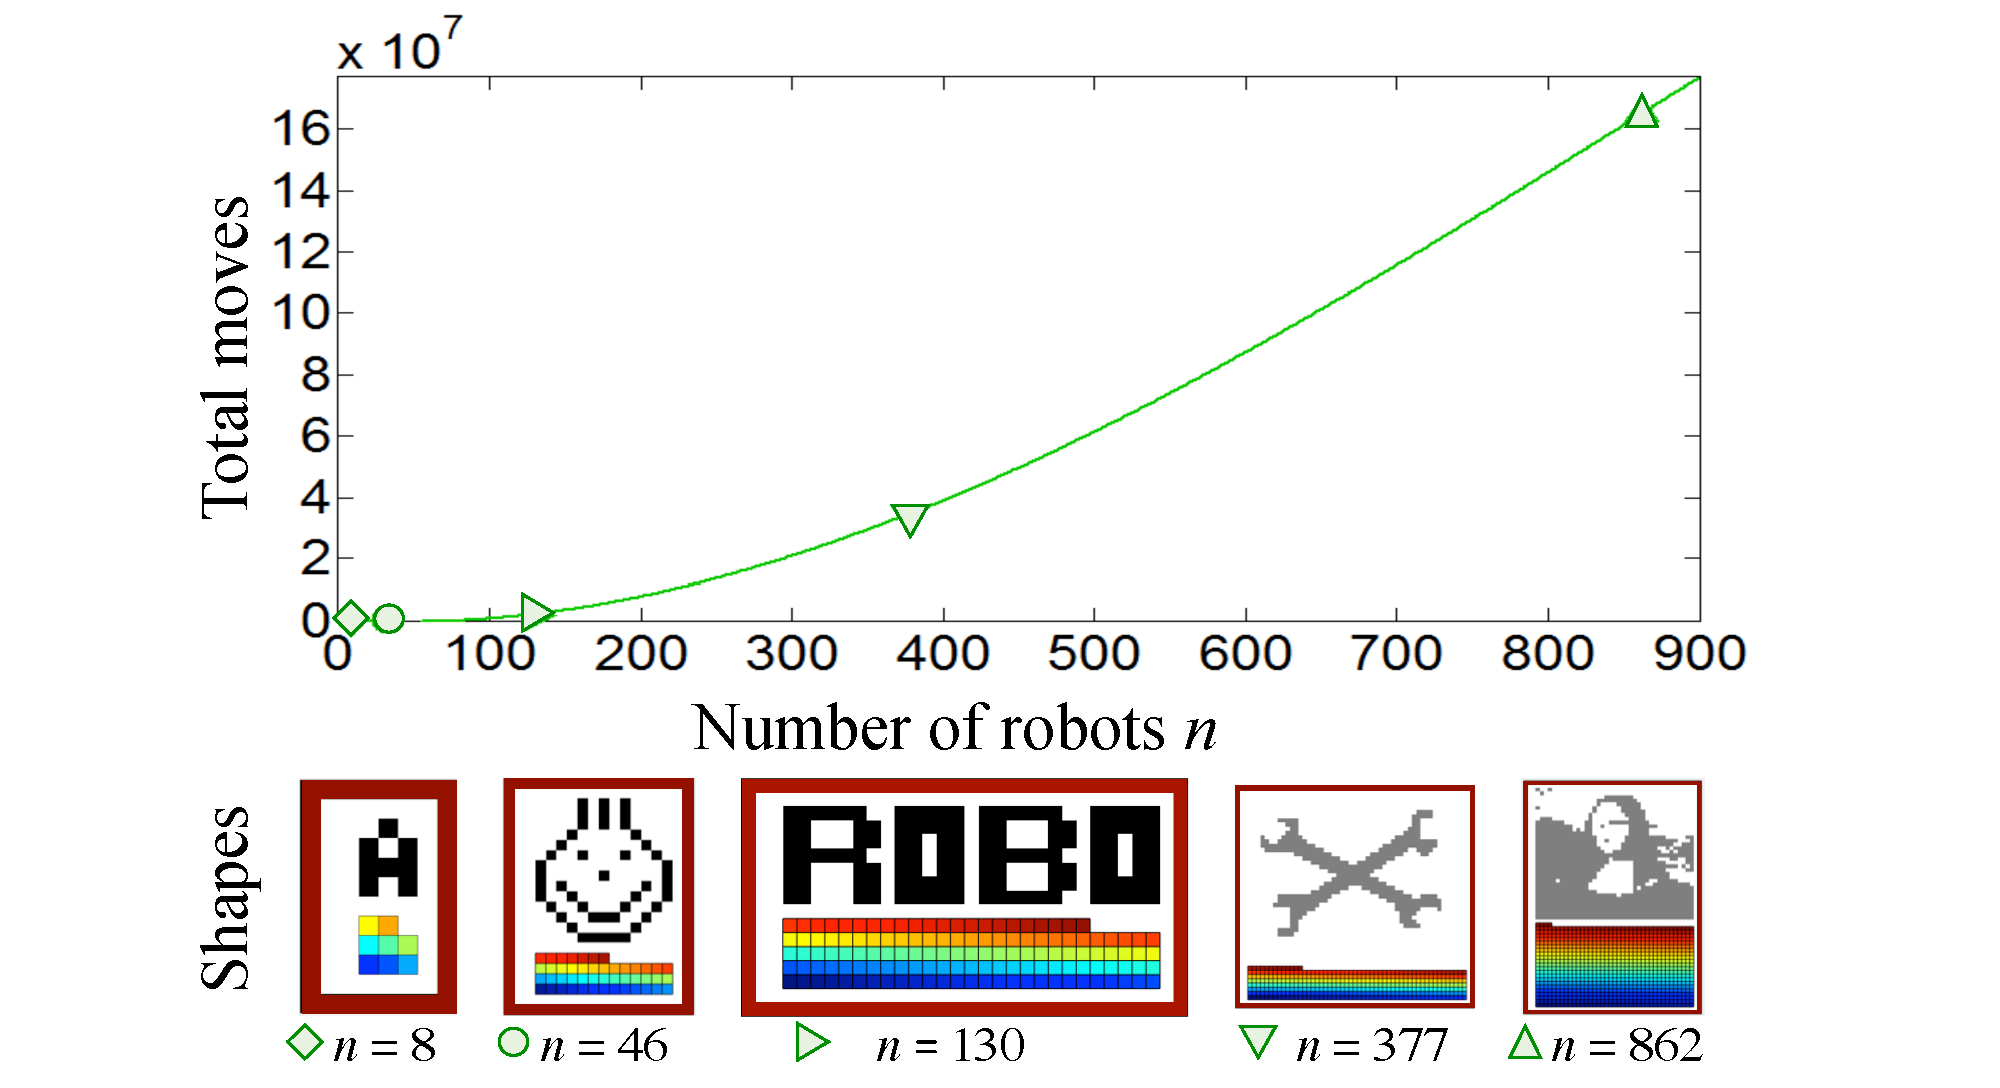
\includegraphics[width=\columnwidth]{5diagramsplots2.pdf}
\end{center}
\vspace{-1em}
\caption{\label{fig:4diagramsplots.pdf}
The required number of moves under Alg. \ref{alg:PosControlNRobots}  using wall-friction to rearrange $n$ square-shaped 
robots.  %The plot compares  \emph{Total distance}---the sum of the moves made by every robot, with \emph{LAP distance}---the shortest distance according to the Linear Assignment Problem using Manhattan distance.  
See hardware implementation and simulation at \citep{Arun2015}.
}
\end{figure}

\begin{figure}
\begin{center}
	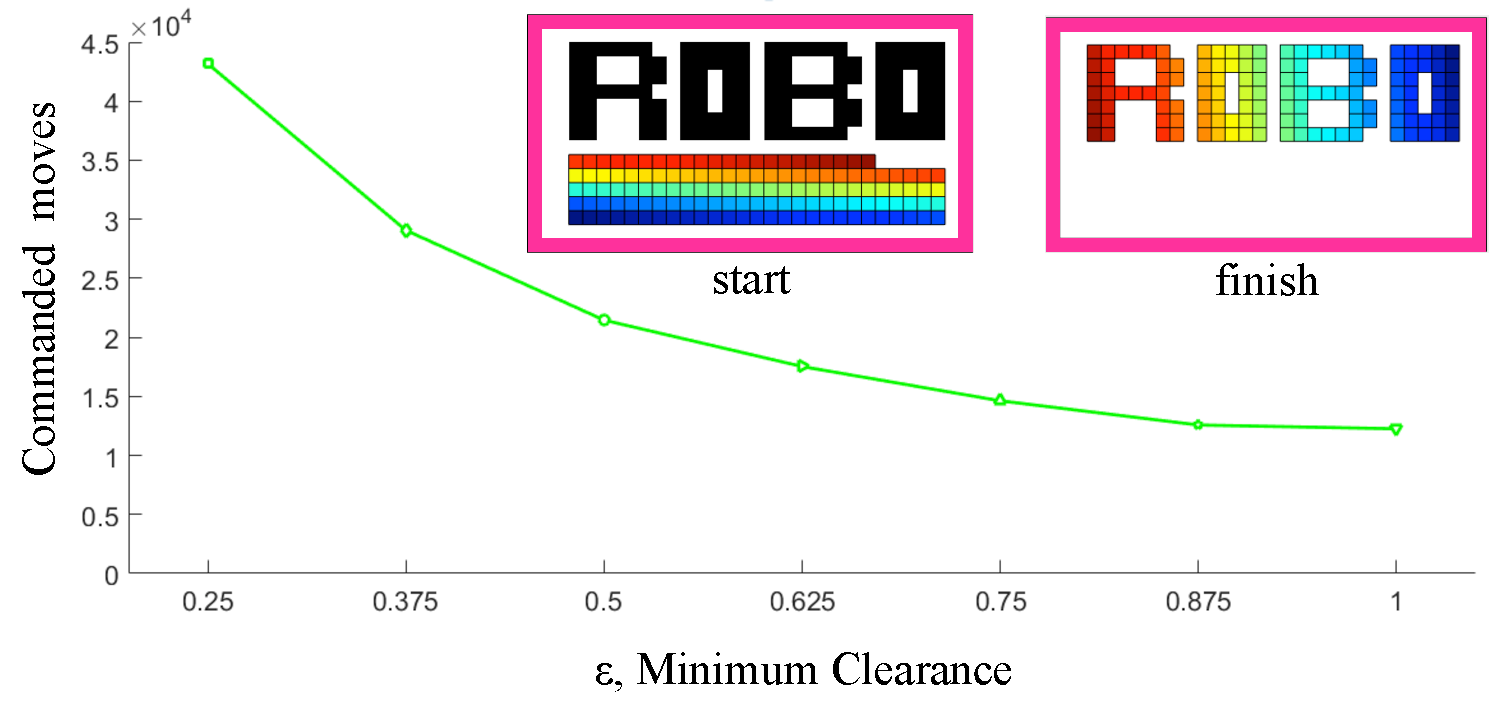
\includegraphics[width=\columnwidth]{graphrobo.pdf}
\end{center}
\vspace{-1em}
\caption{\label{fig:graphrobo.pdf}
Control performance is sensitive to the desired clearance $\epsilon$.  As $\epsilon$ increases, the total distance decreases asymptotically.
}
\end{figure}

\subsection{Efficient Control of Covariance}
%A set of simulations were conducted to demonstrate the importance of boundary friction.  
Random disturbances impair the performance of Alg. \ref{alg:PosControl2Robots} and Alg. \ref{alg:PosControlNRobots}. However, due to the central limit theorem, we can control the covariance of large swarms. This section demonstrates controlling swarm covariance in simulation, using the 2D physics engine Box2D~\citep{catto2010box2d}.
 144 disc-shaped robots with boundary layer model \eqref{eq:boundarylayerflow} were controlled by an open-loop control input as illustrated in Fig. \ref{fig:SimCovarianceFuncFrictionOpenLoop}.  All robots had  the same initial conditions, but in four tests the boundary friction was $F_f = \{0,1/3 F, 2/3F, F\}$.
 Without friction, covariance has minimal variation.  As friction increases, the covariance can be manipulated to greater degrees.


\begin{figure}
\begin{center}
	\includegraphics[width=\columnwidth]{SimCovarianceFuncFrictionOpenLoopV2.pdf}
\end{center}
\vspace{-1em}
\caption{\label{fig:SimCovarianceFuncFrictionOpenLoop}
Open-loop simulation with 144 disc robots and varying levels of boundary friction under the same initial conditions.  Without friction, covariance is unchangeable.  As friction increases, the covariance can be manipulated to greater degrees.
}
\end{figure}

 144 disc-shaped robots were also controlled by a closed-loop controller using the procedure in \S \ref{subsec:ClosedLoopCovarianceControl} with $c_1=0.1$. Fig. \ref{fig:CovVarControlPlot} illustrates that covariance and variances in $x$ and $y$ directions were controlled from a set of initial conditions.
\begin{figure}
\begin{center}
	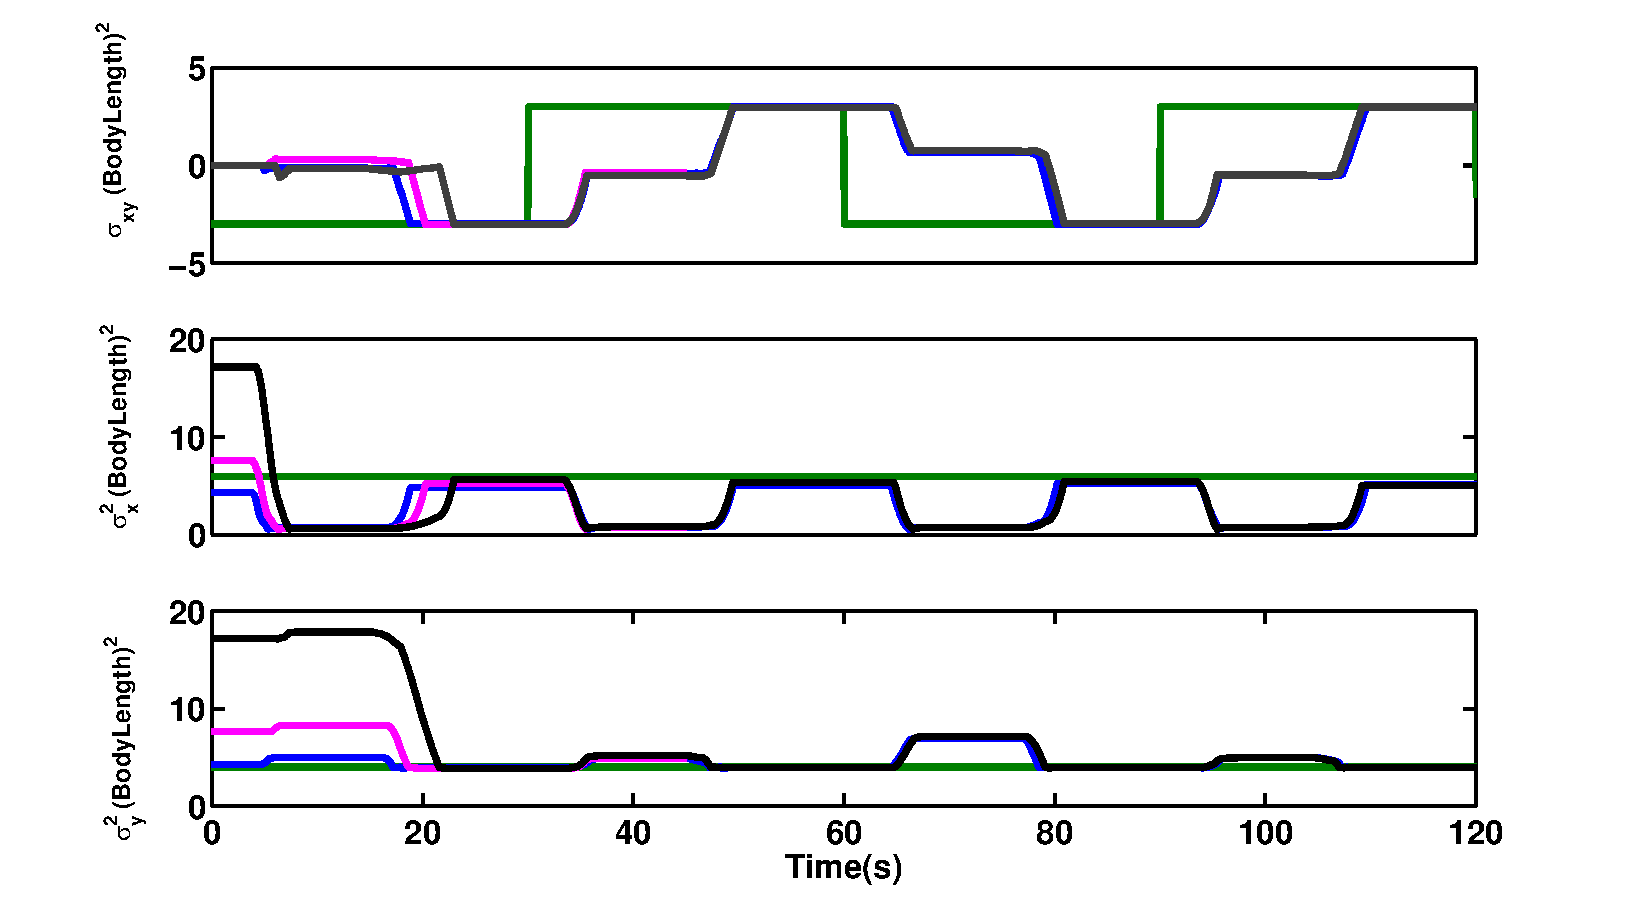
\includegraphics[width=1.0\columnwidth]{CovVarControlPlot2.pdf}
\end{center}
\vspace{-1em}
\caption{\label{fig:CovVarControlPlot}
Closed-loop simulation with 144 disc robots and three sets of initial conditions.  The algorithm tracks goal variance and covariance values (green).  The goal covariance switches sign every 30 s.}
\end{figure}

